% no answer key
\documentclass[letterpaper]{exam}

% answer key
% \documentclass[letterpaper, landscape]{exam}
% \usepackage{2in1, lscape} 
% \printanswers

\usepackage{units} 
\usepackage{graphicx}
\usepackage[fleqn]{amsmath}
\usepackage{cancel}
\usepackage{float}
\usepackage{mdwlist}
\usepackage{booktabs}
\usepackage{polynom}
\usepackage{caption}
\usepackage{fullpage}
\usepackage{comment}
\usepackage{enumerate}
\usepackage{parskip}
\usepackage{xfrac}

\newcommand{\degree}{\ensuremath{^\circ}} 
\everymath{\displaystyle}

% \printanswers
\excludecomment{comment}
\addpoints

\title{Math 142 \\ Chapter One Exam}
\date{\today}
\author{}

\begin{document}

  \maketitle

  \begin{center}
    \gradetable[h][pages]
  \end{center}

  \section{Questions}

  \begin{questions}
    
    \question
      \[
         x = \{ 1, 5, 8, 12, 15 \}
      \]

      \begin{parts}
        \part[2] Find $\bar{x}$.

          \begin{solution}
            $\bar{x} = 8.2$
          \end{solution}

        \part[2] What is the expression for $s_x$?
          \begin{solution}
            \[
              s_x = \sqrt{\frac{(1 - 8.2)^2 + (5 - 8.2)^2 + (8 - 8.2)^2 
                + (12 - 8.2)^2 + (15 - 8.2)^2}{4}}
            \]
          \end{solution}

        % \part[2] What is the value of $s_x$?
        %   \begin{solution}
        %     $s_x \approx 5.5408$
        %   \end{solution}

      \end{parts}

    \question
      \label{q:exams}
      \begin{figure}[H]
        \centering
        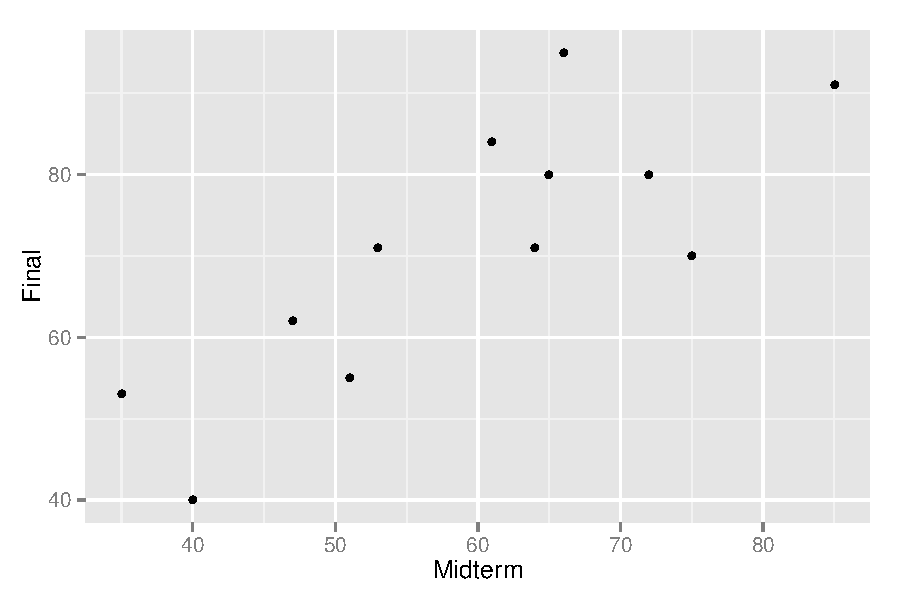
\includegraphics[scale = 0.8]{figures/exams_scatter.pdf}
        \caption{Question \ref{q:exams}}
        \label{fig:exams}
      \end{figure}

      Figure \ref{fig:exams} is a scatter plot of midterm vs. final exam test scores
      for a statistics class.

      \begin{parts}

        \part Estimate the mean score on the final for people who scored more
        than 70 on the midterm:

          \begin{enumerate}[(a)]
            \item about 70
            \item about 80
            \item about 90
          \end{enumerate}

        \part Estimate the correlation coefficient:
          \begin{enumerate}[(a)]
            \item about 0.5
            \item about 0.8
            \item about 0.99
          \end{enumerate}

        \part Draw box plots for the midterm and final
          \ifprintanswers
            \begin{figure}[H]
              \centering
              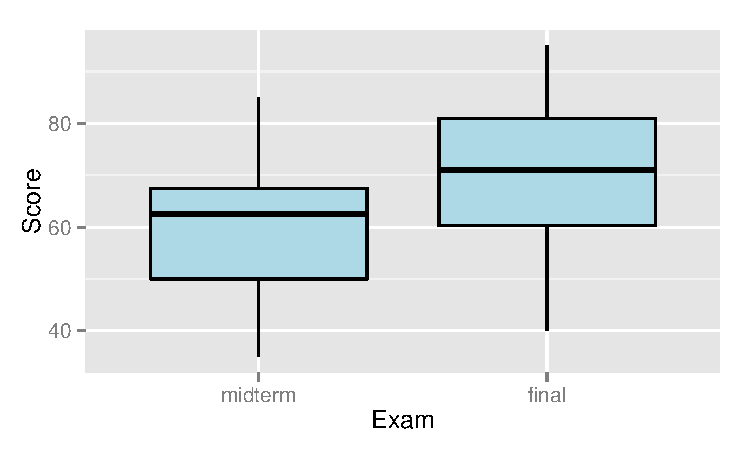
\includegraphics[scale = 0.8]{figures/exams_box.pdf}
              \caption{Question \ref{q:exams}}
              \label{fig:exams_box}
            \end{figure}
          \fi

        \part Was the final exam 
          \begin{enumerate}[(a)]
            \item harder 
            \item easier
            \item about the same difficulty
          \end{enumerate}
          compared to the midterm?

      \end{parts}

    \newpage

    \question
      Here are the average points per game for some NBA starting players:

      \begin{table}[ht]
        \centering
        \begin{tabular}{rlr}
          \toprule
          Player            & Pts/Game \\
          \midrule
          Tayshaun Prince   & 6.10 \\
          Miles Plumlee     & 8.60 \\
          Ricky Rubio       & 8.90 \\
          DeAndre Jordan    & 10.20 \\
          Jonas Valanciunas & 10.40 \\
          Shawn Marion      & 10.50 \\
          Terrence Jones    & 11.80 \\
          Channing Frye     & 11.80 \\
          Tristan Thompson  & 12.20 \\
          Jameer Nelson     & 12.30 \\
          Andre Drummond    & 13.10 \\
          Carlos Boozer     & 14.30 \\
          Gerald Henderson  & 14.60 \\
          Jodie Meeks       & 14.80 \\
          Jeff Teague       & 16.10 \\
          Bradley Beal      & 16.90 \\
          Evan Turner       & 17.40 \\
          David Lee         & 18.60 \\
          Monta Ellis       & 18.90 \\
          Damian Lillard    & 20.80 \\
          Paul George       & 22.20 \\
          Stephen Curry     & 23.60 \\
          LeBron James      & 27.20 \\
          Carmelo Anthony   & 28.10 \\
          Kevin Durant      & 31.80 \\
          \bottomrule
        \end{tabular}
      \end{table}

      \begin{parts}
        \part[10] Draw a histogram with a bin width of 5 points for these players.

        \part[2] Is the distribution symmetrical, left-skewed, or right-skewed?

        \part[5] Without calculating either one, is the mean score to be higher or
        lower than the median?  Explain why you don't need to do any calculations to
        answer this question.

        \part[3] Is the median or mean a better measure of the center of this
          distribution?  Why?

      \end{parts}

    \newpage

    \question
      There is heated debate this year about whether Kevin Durant or
      LeBron James should be the MVP.  

      Here is a random but representative selection of their per game point totals
      this season:

      \begin{tabular}[H]{ll}
        Durant & \{ 13, 17, 19, 24, 26, 28, 29, 31, 32, 32, 32, 37, 41, 42, 42 \} \\
        James  & \{ 13, 15, 17, 19, 25, 25, 25, 26, 29, 30, 32, 33, 35, 36, 36 \} \\ 
      \end{tabular}

      \begin{parts}
        \part[6] Find the 5-number summary for both players
        \part[6] Draw a box plot for both players
        \part[3] Which player seems to be the MVP, based solely on points scored?
      \end{parts}

    \question
      The MVP award is about how much you help your team, particularly in close
      games.  Tables \ref{tab:durant_diff} and \ref{tab:james_diff} show the points
      scored by each player in games which were decided by less than 5 points.  The
      ``Final Score'' is the difference between Durant/James team and the score of
      whoever they were playing.

      The correlation coefficients and standard deviations are:

      \begin{table}[ht]
        \centering
        \begin{tabular}{rr}
          \toprule
          Points & Final Score \\
          \midrule
          42     & 3 \\
          33     & 1 \\
          20     & -1 \\
          38     & 2 \\
          25     & 1 \\
          27     & 2 \\
          28     & 3 \\
          34     & 4 \\
          37     & -4 \\
          24     & -2 \\
          48     & 4 \\
          37     & -3 \\
          41     & 2 \\
          29     & -1 \\
          36     & 3 \\
          43     & 4 \\
          \bottomrule
        \end{tabular}
        \caption{Durant points and final score differential}
        \label{tab:durant_pt_diff}
      \end{table}

      \begin{table}[ht]
        \centering
        \begin{tabular}{rrr}
          \toprule
          Points & Final Score \\
          \midrule
          25     & -1 \\
          22     & -3 \\
          31     & 4 \\
          26     & 3 \\
          24     & 3 \\
          36     & 1 \\
          26     & 1 \\
          38     & 2 \\
          25     & -4 \\
          22     & 2 \\
          \bottomrule
        \end{tabular}
        \caption{James points and final score differential}
        \label{tab:james_pt_diff}
      \end{table}

      \begin{parts}
        \part[10] Make a scatter plot for each player using points as the explanatory
          variable and point differential as the response variable.

        \part[10] Find the equation for the regression line for each player and add
        regression lines to the two scatter plots.

        \part[3] If LeBron scores 30 points in a close game, what would you expect
        his team's margin of victory to be?

        \part[2] How confident can you be in the accuracy of the prediction from part c?

        \part[3] Based on this analysis, which player deservers the MVP award?
      \end{parts}

      \question
        Tables \ref{tab:durant_pt_diff} and \ref{tab:james_pt_diff} can also be used
        to predict how many points the two players would need to score in order to
        win a close game.

        \begin{parts}
          \part[5]
            Find the equation for the regression line for Kevin Durant with the final
            score as the explanatory variable and Durant's parts as the response
            variable.

          \part[5] Use the regression line to determine about how many points Durant would
          need to score in order for his team to win a close game by 2 points.

          \part[2] How confident can you be in the accuracy of the prediction from 
            part b?
        \end{parts}
        
      \question
        Three point shooting accuracy in 2013 is a roughly Normal distribution with a
        mean of 0.36 and a standard deviation of 0.05.

        \begin{parts}
          \part[5] Carmelo Anthony's three point shooting accuracy is 0.42 this
          year.  What is the z-score for this value?

          \begin{solution}
            \[
              \frac{0.42 - 0.36}{0.05} \approx \boxed{ 1.2 }
            \]
          \end{solution}

          \part[5] Use Table A to find what percentage of the three point shooters
            in the NBA are less accurate than Melo.
            \begin{solution}
              about 0.8849 or 88.5\%
            \end{solution}
        \end{parts}
        
  \end{questions}
\end{document}

